% Replace the author placeholders below before submission.
% Compile with: pdflatex clustering_report.tex (twice for stable references).
\documentclass[conference]{IEEEtran}

\usepackage{graphicx}
\usepackage{booktabs}
\usepackage{array}
\usepackage{cite}
\usepackage{url}

% BasicTeX does not include the optional Courier font metrics by default.
\renewcommand{\ttdefault}{cmtt}

\graphicspath{{figures/}}
\setlength{\textfloatsep}{5pt plus 1pt minus 1pt}
\setlength{\floatsep}{4pt plus 1pt minus 1pt}
\setlength{\intextsep}{5pt plus 1pt minus 1pt}

\title{Clustering Urban Mobility Patterns Using Bike-Sharing Data}

\author{\IEEEauthorblockN{\mbox{J. U. P. Lelwala}}
\IEEEauthorblockA{\mbox{230374E}}}

\begin{document}
\maketitle

\begin{abstract}
This study identifies recurring daily mobility regimes in the Capital Bikeshare system using 17,379 hourly observations from 2011--2012. Hourly records were converted into 731 daily mobility vectors, cleaned, checked for incomplete days, and summarized using demand, peak-period, user-composition, and environmental features. K-means, agglomerative hierarchical clustering (AGNES), and DBSCAN were compared through internal validity, separation, compactness, balance, coverage, and stability. Four-cluster K-means provided the best overall compromise, separating warm and cool conditions while independently distinguishing commuter and leisure behaviour. The resulting profiles support differentiated rebalancing, capacity, maintenance, and seasonal planning strategies.
\end{abstract}

\begin{IEEEkeywords}
bike sharing, clustering, K-means, AGNES, DBSCAN, urban mobility
\end{IEEEkeywords}

\section{Introduction and Data}
Bike-sharing demand changes with the work calendar, season, weather, and user type. Discovering recurrent daily patterns can help operators anticipate bicycle availability and schedule rebalancing or maintenance. This work uses the UCI Bike Sharing Dataset \cite{uci}, containing Capital Bikeshare hourly demand and environmental observations for Washington, D.C. \cite{fanaee}. The clustering unit is a day rather than an individual hour.

The hourly file contains 17,379 rows, 17 columns, and 731 dates. No missing cell values, exact duplicates, duplicate date-hour keys, invalid category codes, negative counts, or violations of \(\texttt{casual}+\texttt{registered}=\texttt{cnt}\) were found. Daily totals reconstructed from the hourly file matched the supplied daily reference exactly.

Only 655 days contained 24 recorded hours; 76 were incomplete, with 165 absent date-hour combinations. Since all recorded hourly counts were positive and the daily totals reconciled, absent hours were represented as zero demand in a separate 24-hour grid. Observed rows were retained for environmental averages. No day was manually deleted. The eight days with fewer than 20 observed hours were flagged for sensitivity and anomaly interpretation, including the Hurricane Sandy period.

\section{Feature Engineering and Exploration}
Each date was represented by total, mean, maximum, and standard deviation of hourly rentals; morning (06:00--09:00), evening (16:00--19:00), and off-peak shares; casual and registered proportions; and mean temperature, humidity, and wind speed. The 24-hour grid was used for demand-shape statistics, while observed measurements were used for weather averages.

No feature had absolute skewness above 1, so no power or logarithmic transformation was applied. Redundancy checks showed that mean demand equals total demand divided by 24, casual and registered proportions sum to one, and the three period shares sum to one. Total demand was also highly correlated with maximum demand and hourly variability. The final clustering vector retained seven features: total rentals, morning share, evening share, casual proportion, temperature, humidity, and wind speed. All were standardized to zero mean and unit population variance.

Exploration showed strong commuting peaks on working days and broad midday demand on non-working days. Demand was generally higher in 2012 and in warmer periods. The first two principal components explained 56.6\% of standardized variance; PCA was therefore used for visualization only, while clustering used all seven dimensions.

\section{Clustering Methods}
\subsection{K-means}
K-means was fitted for \(k=2,\ldots,10\) using 50 initializations and random seed 42. Inertia displayed an elbow around \(k=4\) (Fig.~\ref{fig:kselect}). Although \(k=2\) had the highest silhouette score, it produced only a broad commuter-versus-leisure division. The four-cluster solution had a better silhouette than the adjacent \(k=3\) and \(k=5\) solutions and provided distinct operational regimes.

\begin{figure}[t]
\centering
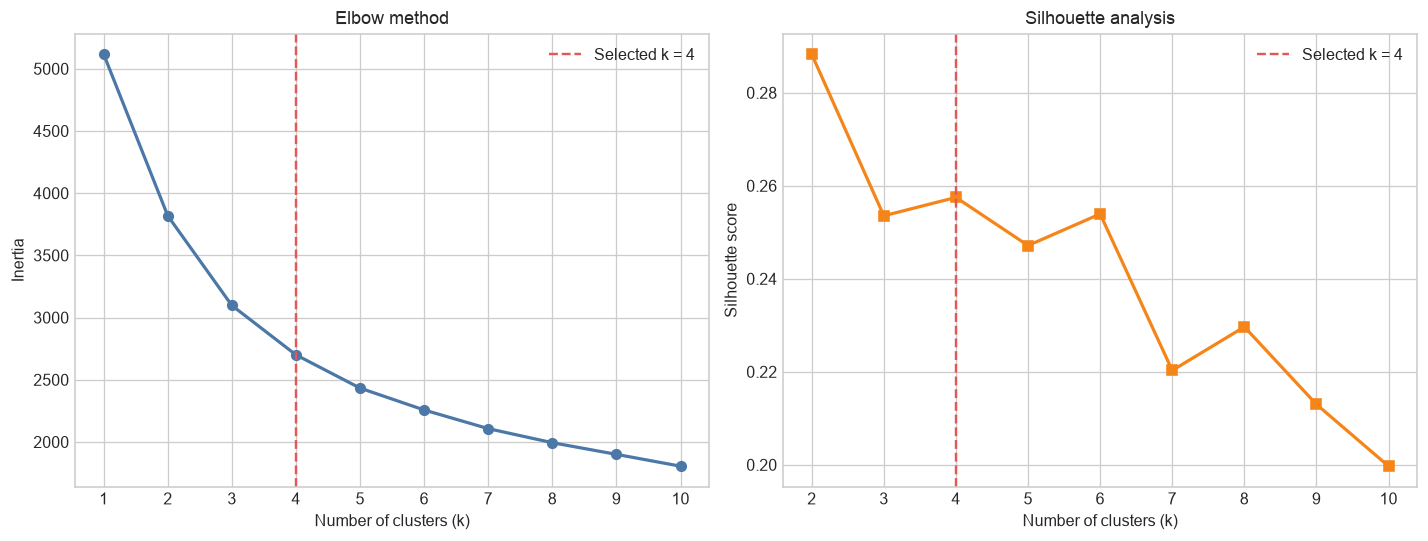
\includegraphics[width=\columnwidth]{kmeans-selection.png}
\caption{Elbow and silhouette evidence for K-means selection.}
\label{fig:kselect}
\end{figure}

\subsection{AGNES}
AGNES was applied with Euclidean distance and single, complete, and average linkage. Dendrogram cuts from two to ten clusters were evaluated using silhouette, Davies-Bouldin, and size balance. Single linkage exhibited chaining: its two-cluster cut contained 729 and 2 days. Average linkage similarly isolated tiny groups. Complete linkage at three clusters was the most meaningful hierarchical result, producing sizes 373, 356, and 2, although the two-day branch still indicated strong sensitivity to extreme observations.

\subsection{DBSCAN}
The density threshold was investigated using sorted 14-nearest-neighbour distances, where \(\texttt{min\_samples}=2d=14\) for \(d=7\). The geometric knee near \(\epsilon=1.92\) merged almost all observations. A lower shoulder, \(\epsilon=1.30\), retained meaningful density structure: three clusters of 426, 103, and 34 days plus 168 noise points. Alternatives \(\epsilon=1.20\), \(1.40\), and \(\texttt{min\_samples}=10\) confirmed sensitivity in both cluster and noise counts. Seven of eight severely incomplete days were noise, but validation showed these were not automatically data errors; several represented genuine disruption or rare-demand conditions.

\section{Evaluation and Method Selection}
Table~\ref{tab:evaluation} compares final solutions in standardized Euclidean space. Mean intra-cluster distance uses pairs within the same cluster, while inter-cluster distance uses pairs with different labels. For DBSCAN, noise was excluded from silhouette, Davies-Bouldin, and distance calculations but retained in coverage and size reporting.

\begin{table}[t]
\caption{Internal Evaluation of Final Clusterings}
\label{tab:evaluation}
\centering
\scriptsize
\resizebox{\columnwidth}{!}{%
\begin{tabular}{lrrrrrr}
\toprule
Method & Sil. & DB & Intra & Inter & Ratio & Coverage \\
\midrule
K-means (4) & 0.257 & 1.457 & 2.474 & 3.960 & 1.600 & 100\% \\
AGNES complete (3) & 0.115 & 1.952 & 3.296 & 3.779 & 1.147 & 100\% \\
DBSCAN (3) & 0.296 & 1.015 & 2.571 & 3.916 & 1.523 & 77\% \\
\bottomrule
\end{tabular}}
\end{table}

K-means cluster sizes were 107, 274, 130, and 220, giving normalized balance entropy 0.950. AGNES balance was 0.646 because of its two-day group. DBSCAN balance was 0.629 among clustered observations and left 23\% as noise. Stability was measured by adjusted Rand index (ARI). K-means achieved mean ARI 0.990 across 20 seeds; DBSCAN averaged 0.816 across nearby parameter settings; AGNES averaged 0.253 across linkage and cut perturbations.

DBSCAN obtained the strongest silhouette and Davies-Bouldin scores only after excluding 168 days. AGNES was poorly balanced and linkage-sensitive. K-means was selected because it combined full coverage, the largest inter/intra ratio, the best balance, high stability, and interpretable regimes. Its forced assignment of unusual days remains a limitation; DBSCAN noise labels were retained as supporting anomaly evidence.

\section{Cluster Interpretation and Insights}
Table~\ref{tab:profiles} reports original-scale profiles. Calendar and weather variables were not clustering inputs, so their distributions provide external validation. Clusters 1 and 3 were 98.9\% and 99.5\% working days. Clusters 0 and 2 were 83.2\% and 93.1\% weekends. Warm high-demand clusters were concentrated in summer/fall, while cool clusters were concentrated in spring/winter. The contextual separation is summarized in Fig.~\ref{fig:context}.

\begin{table}[t]
\caption{Original-Scale Profiles of Selected Clusters}
\label{tab:profiles}
\centering
\scriptsize
\resizebox{\columnwidth}{!}{%
\begin{tabular}{clrrrrr}
\toprule
C & Description & Days & Total & Morn. & Eve. & Casual \\
\midrule
0 & Cool low-demand weekends & 107 & 2471 & .082 & .249 & .204 \\
1 & Warm high-demand commuters & 274 & 5757 & .228 & .369 & .155 \\
2 & Warm high-demand leisure & 130 & 5653 & .075 & .279 & .357 \\
3 & Cool registered commuters & 220 & 3254 & .268 & .347 & .080 \\
\bottomrule
\end{tabular}}
\end{table}

Cluster 1 requires the greatest peak capacity: bicycles should be positioned before morning commuting and rebalanced toward residential areas before the evening return peak. Cluster 3 needs the same timing pattern at lower cool-season volume. Cluster 2 requires a different weekend plan, with capacity shifted toward recreational and tourist destinations around its broad midday plateau. Cluster 0 offers the best planned-maintenance window because demand is lowest, although a minimum weekend service level is still required. Weather forecasts should be combined with the work calendar to distinguish high-demand commuter days from equally busy leisure days. Exact station movements require station-level origin, destination, or inventory data, which this dataset does not provide.

\begin{figure*}[t]
\centering
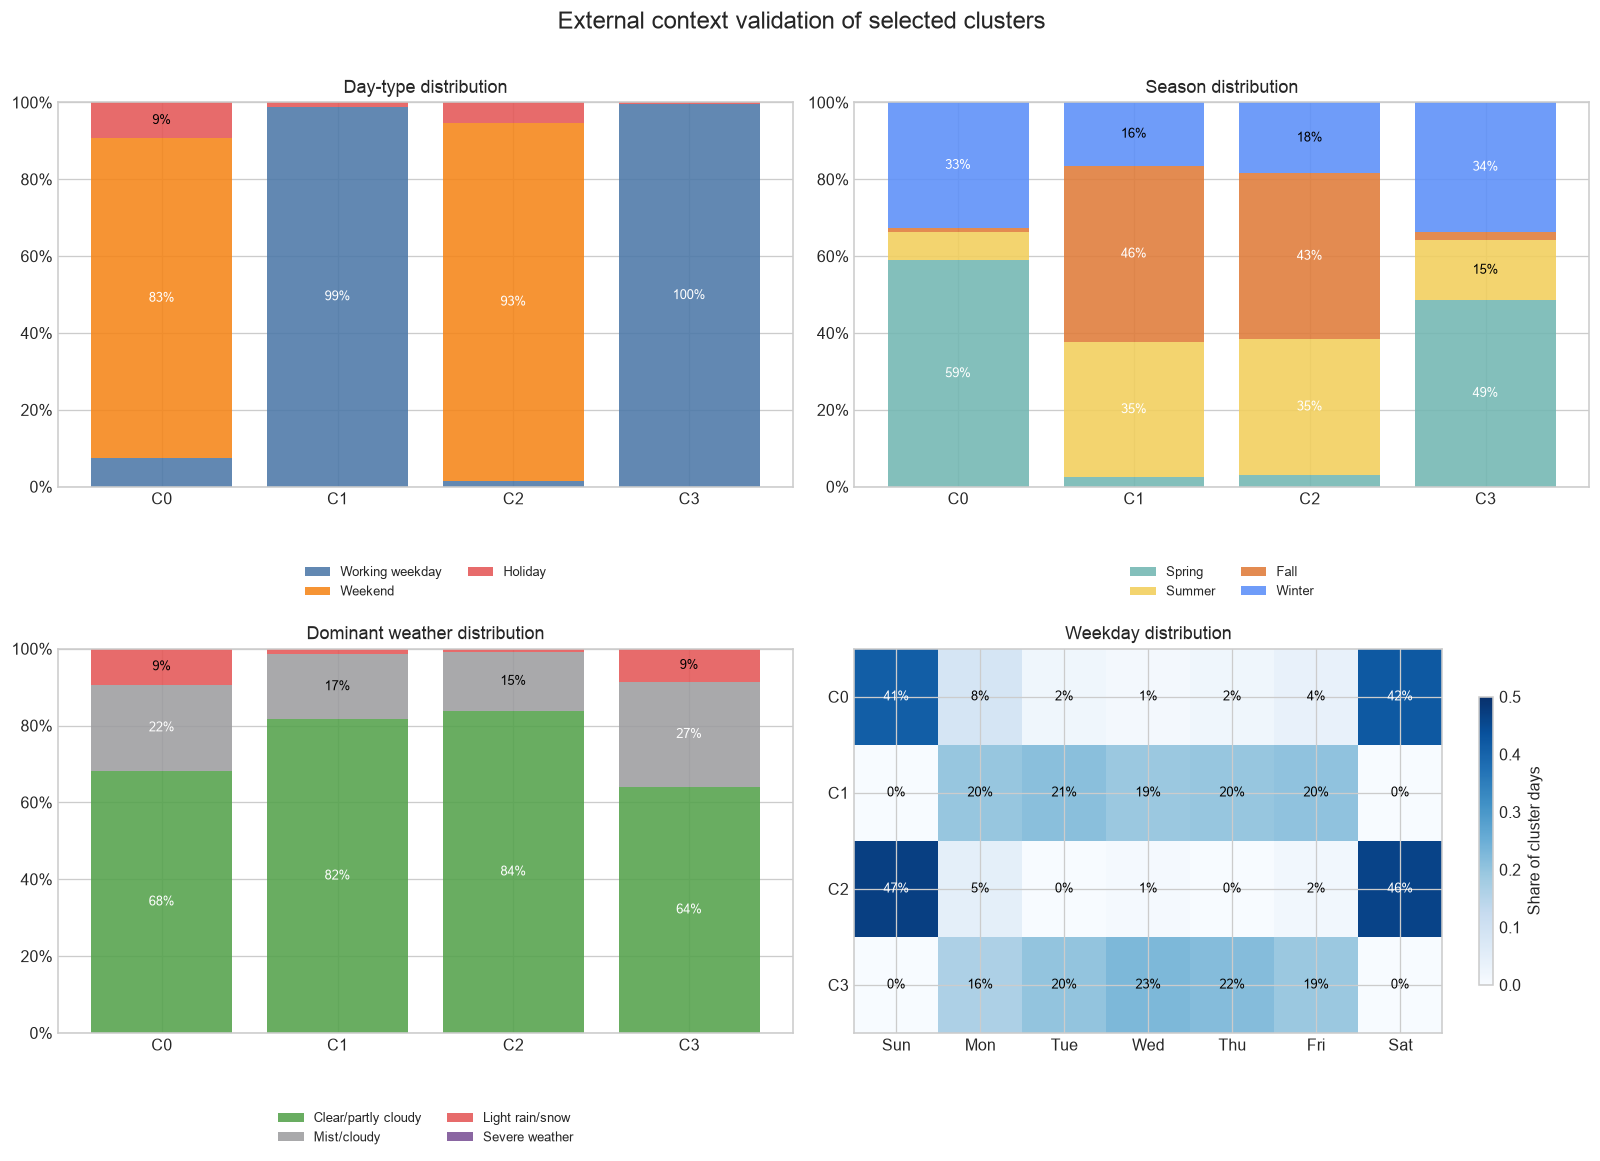
\includegraphics[width=0.88\textwidth]{cluster-context.png}
\caption{External validation using day type, season, dominant weather, and weekday distributions.}
\label{fig:context}
\end{figure*}

\section{Theoretical Understanding}
\begin{enumerate}
\setlength{\itemsep}{1pt}
\setlength{\parskip}{0pt}
\item \textbf{K-means assumptions.} K-means favours compact, convex, approximately spherical clusters under Euclidean distance. It works best when clusters have comparable spread and size; centroids and squared distances make it sensitive to outliers.

\item \textbf{Effect of linkage.} Single linkage uses the nearest cross-cluster pair and can preserve irregular shapes. Complete linkage uses the farthest pair and favours compact groups. Average linkage is intermediate and compares mean cross-cluster distance.

\item \textbf{Single-link chaining.} A single close pair is sufficient to merge two groups. Repeated bridges of intermediate observations can therefore create a long chain even when most members are far apart.

\item \textbf{DBSCAN noise versus K-means assignment.} DBSCAN requires enough neighbours inside an \(\epsilon\)-radius; points outside dense regions can remain noise. K-means minimizes a partition objective and must assign every observation to its nearest centroid.

\item \textbf{Need for scaling.} Rental totals are measured in thousands, while shares and weather variables are near zero to one. Without standardization, count variables would dominate Euclidean distances and the resulting clusters.

\item \textbf{Correlated features.} Highly correlated variables repeatedly encode the same direction, implicitly increasing its weight in distance calculations. This can distort separation and hide weaker but meaningful dimensions.

\item \textbf{PCA for visualization only.} A two-dimensional PCA view is simple and preserves the largest-variance directions, but may hide separation in later components. Clustering the full standardized data avoids information loss; clustering PCA scores can instead reduce noise and collinearity but depends on the number of retained components.

\item \textbf{Manhattan versus Euclidean distance.} Manhattan distance forms diamond-shaped neighbourhoods and is less dominated by a few large coordinate deviations. Assignments may change for elongated or outlier-prone data. Standard K-means is tied to squared Euclidean distance, so a Manhattan objective should use a k-medians-type method.

\item \textbf{Why multiple metrics are required.} Metrics reward different properties and have different biases regarding shape, size, density, and noise. High separation can coexist with imbalance, instability, poor coverage, or weak practical meaning.

\item \textbf{Valid unusual day versus data-quality outlier.} A valid unusual day passes structural checks but reflects a real event such as severe weather, a closure, or a holiday. A data-quality outlier arises from invalid values, duplication, missing capture, or inconsistent totals and should be resolved using provenance rather than score improvement.
\end{enumerate}

\section{Reproducibility and Conclusion}
The analysis used Python 3.14.3, pandas 3.0.5, NumPy 2.5.1, scikit-learn 1.9.0, SciPy 1.18.0, and Matplotlib 3.11.1. K-means used seed 42 and 50 initializations. All cleaning decisions and parameter alternatives are executable from top to bottom in the accompanying notebook.

Four stable and operationally meaningful K-means regimes were identified. Their independent alignment with the work calendar and season supports the interpretation that daily bike-sharing demand is governed jointly by activity purpose and environmental conditions, rather than demand magnitude alone.

\begin{thebibliography}{00}
\bibitem{uci} H. Fanaee-T, ``Bike Sharing Dataset,'' UCI Machine Learning Repository, 2013. [Online]. Available: \url{https://archive.ics.uci.edu/dataset/275/bike+sharing+dataset}
\bibitem{fanaee} H. Fanaee-T and J. Gama, ``Event labeling combining ensemble detectors and background knowledge,'' \emph{Progress in Artificial Intelligence}, 2013, doi: 10.1007/s13748-013-0040-3.
\bibitem{ester} M. Ester, H.-P. Kriegel, J. Sander, and X. Xu, ``A density-based algorithm for discovering clusters in large spatial databases with noise,'' in \emph{Proc. KDD}, 1996, pp. 226--231.
\bibitem{silhouette} P. J. Rousseeuw, ``Silhouettes: A graphical aid to the interpretation and validation of cluster analysis,'' \emph{J. Comput. Appl. Math.}, vol. 20, pp. 53--65, 1987.
\bibitem{dbindex} D. L. Davies and D. W. Bouldin, ``A cluster separation measure,'' \emph{IEEE Trans. Pattern Anal. Mach. Intell.}, vol. PAMI-1, no. 2, pp. 224--227, 1979.
\end{thebibliography}

\end{document}
